\section{State of the Union Addresses}
The main textual data that was collected to be processed was all of the Presidential State of the Union addresses, from George Washington's first address to Barack Obama's last address.
The text source was initially pulled from a Presidential Address Repository [\cite{presrepo}].
The text came in a large text file that contained every speech and it was split in to individual text files for each individual address to allow for easier processing.
The addresses vary widely in length and content, which is also of significant note when analyzing and comparing these addresses across the timespan of the existence of the United States.
George Washington's first address was just over a thousand words and seventeen paragraphs, whereas Barack Obama's final address was just over 5,400 words and was 78 paragraphs long.

\subsection{Change in Purpose of State of the Union Address}
The length is the most notable change in the State of the Union Addresses over time, but there are important factors to consider as well that could potentially impact how the addresses are given from year to year.
When the Presidential Addresses first started with George Washington, it was not intended to be a recurring event [\cite{teten2003evolution}], but it soon began to grow to a tradition so that the president could publicly address the people and inform them of the current events of the country.
Over the years, the Presidential Address has taken on many forms, in spoken word, in written letter, in radio broadcast, and, nowadays, on live television broadcast.
The Presidential Address shifted from the yearly Presidential update, sometimes the only time people would hear directly from the President, to a formalized briefing to inform the public in an organized manner of the current state of affairs and push forward a President's agenda for the upcoming term [\cite{teten2003evolution}].
While that has always been a goal of the addresses, it has become more of the central focus over the course of time, due to technological innovations and changes in media coverage.
Nowadays, citizens of the United States can read in real-time about the decisions of the Presidency and the Presidents political moves without needing to listen to an annual speech to become updated on their agenda and goals for the year to come.
It is a subtle, yet interesting shift in how the addresses are approached, but even these purposes could change, depending on the person giving these orations, an important factor to consider also.

\subsection{Presidential Personality}
Another important factor in how the Presidential State of the Union Addresses are given is the personality of the President that is giving them.
This is a rather intangible element of the speeches that can be hard to quantify but is very important to note.
Most people have a certain disposition towards being more optimistic or pessimistic, and that can become apparent in the speeches given.
The important topic being considered here is tone, which can be heavily influenced if the President giving the speech tends to be more realistic or optimistic in their outlook on the world.
Some President's may see the State of the Union as a chance to rally the nation and project positivity and support for their platform for years to come, whereas others might see it as a good opportunity to have a nation-wide reality check and bring the citizens in-line with what needs to be done for the good of the nation [\cite{teten2003evolution}].

\section{Statistical Summary}
It is important to have an understanding of the speech data itself before diving in to this research, since otherwise it won't be as meaningful and it will be harder to draw conclusions.
The full statistical summary for the data can be found in Table \ref{stat:one}.
This can be explored to search for trends in the data and familiarize oneself with an overall perspective on the data.
Some information of note: 
There are a total of 230 Presidential Addresses given by 42 Presidents, making the average number of addresses per president 5. 
There are 26 Republicans and 16 Democrats, which makes their percentages 62\% and 38\%, respectively.
The first three columns are self-explanatory and the latter two are described below.

\subsection{Lexical Diversity}
Lexical diversity is a metric that is used to represent the amount of unique words in any given passage of text and thus the overall complexity of the text [\cite{johansson2009lexical}].
Lexical diversity is calculated by dividing the number of unique words in a text by the total length of the text.
The resulting number is between 0 and 1 and the closer to 1, the more diverse the lexicon, so a value close to 1 can be interpreted as being more complicated to read.
The patterns here can be confounding by sheer length of a text but it remains an important metric to see how complex a particular selection of text is.
The nature of this calculation makes it more interesting when comparing two pieces of text that are similar in length to see the lexical diversity between the two.
This calculation was performed for each State of the Union address and then all of the scores for each President were averaged together to get an average lexical diversity for each President.

\subsection{Grade Level}
Calculating grade level is a slightly more involved process that involves an algorithm that computes grade level based on two factors: average sentence length and average syllables per word.
This formula was created in 1975 to determine the readability of documents for Navy enlisted personnel [\cite{kincaid1975derivation}]
The first factor is relatively easy to calculate, but the second is slightly more tricky as syllables can be a lot more difficult to distinguish in plain text processing fashion.
Luckily, there is a Python plugin called textstat with a built-in Flesch-Kincaid function that has a corpus of syllabled words and it was used to calculate grade level.
You can see how the formula is used in Equation \ref{eq1}.

\begin{equation} \label{eq1}
    0.39\ (\frac{total\ words}{total\ sentences}) + 11.8\ (\frac{total\ syllables}{total\ words}) - 15.59
\end{equation}

\begin{singlespace}
\begin{table}[tp]
\begin{center}
 \begin{tabular}{||c | c c c c||}
 \hline
 President & \# of Addrs. & Avg \# Words & Lex Diversity & Grade Level \\
 \hline\hline
 George Washington & 8 & 2096.0 & 0.3762 & 18.55 \\ 
 \hline
 John Adams & 4 & 1801.0 & 0.369 & 17.925 \\
 \hline
 Thomas Jefferson & 8 & 2605.0 & 0.3376 & 18.0 \\
 \hline
 James Madison & 8 & 2729.0 & 0.3433 & 20.825 \\
 \hline
  James Monroe & 8 & 5326.0 & 0.2493 & 16.462 \\
 \hline
  John Quincy Adams & 4 & 7864.0 & 0.2327 & 19.25 \\
 \hline
  Andrew Jackson & 8 & 10708.0 & 0.2042 & 19.2 \\
 \hline
  Martin van Buren & 4 & 11411.0 & 0.2036 & 20.15 \\
 \hline
  John Tyler & 4 & 8560.0 & 0.2291 & 18.475 \\
 \hline
  James Polk & 4 & 18173.0 & 0.1525 & 17.275 \\
 \hline
  Zachary Taylor & 1 & 7678.0 & 0.2346 & 17.2 \\
 \hline
  Millard Fillmore & 3 & 10612.0 & 0.2224 & 16.967 \\
 \hline
  Franklin Pierce & 4 & 10545.0 & 0.2192 & 19.15 \\
 \hline
  James Buchanan & 4 & 14247.0 & 0.1797 & 15.05 \\
 \hline
  Abraham Lincoln & 4 & 6999.0 & 0.2639 & 13.675 \\
 \hline
  Andrew Johnson & 4 & 9690.0 & 0.2294 & 15.9 \\
 \hline
  Ulysses S. Grant & 8 & 8232.0 & 0.2391 & 15.938 \\
 \hline
  Rutherford B. Hayes & 4 & 8692.0 & 0.2363 & 16.325 \\
 \hline
  Chester A. Arthur & 4 & 5045.0 & 0.3252 & 13.6 \\
 \hline
  Grover Cleveland & 4 & 12478.0 & 0.2236 & 17.45 \\
 \hline
  Benjamin Harrison & 4 & 13881.0 & 0.1976 & 14.7 \\
 \hline
  Grover Cleveland & 4 & 14969.0 & 0.2121 & 16.35 \\
 \hline
  William McKinley & 4 & 16901.0 & 0.1977 & 15.8 \\
 \hline
  Theodore Roosevelt & 8 & 19793.0 & 0.1732 & 14.975 \\
 \hline
  William H. Taft & 4 & 17594.0 & 0.1868 & 17.025 \\
 \hline
  Woodrow Wilson & 8 & 4384.0 & 0.2768 & 15.05 \\
 \hline
  Warren Harding & 2 & 5738.0 & 0.2768 & 13.5 \\
 \hline
  Calvin Coolidge & 6 & 8707.0 & 0.2306 & 11.783 \\
 \hline
  Herbert Hoover & 4 & 6489.0 & 0.2566 & 14.15 \\
 \hline
  Franklin D. Roosevelt & 12 & 3991.0 & 0.3002 & 12.0 \\
 \hline
  Harry S. Truman & 8 & 8405.0 & 0.2321 & 10.475 \\
 \hline
  Dwight D. Eisenhower & 9 & 6103.0 & 0.2751 & 12.3 \\
 \hline
  John F. Kennedy & 3 & 5816.0 & 0.289 & 12.233 \\
 \hline
  Lyndon B. Johnson & 6 & 4917.0 & 0.2707 & 10.017 \\
 \hline
  Richard Nixon & 5 & 4002.0 & 0.2692 & 11.78 \\
 \hline
  Gerald R. Ford & 3 & 4649.0 & 0.2865 & 10.767 \\
 \hline
  Jimmy Carter & 4 & 11410.0 & 0.2427 & 11.05 \\
 \hline
  Ronald Reagan & 7 & 4731.0 & 0.2963 & 9.557 \\
 \hline
  George H.W. Bush & 4 & 4396.0 & 0.285 & 7.8 \\
 \hline
  Bill Clinton & 8 & 7528.0 & 0.2207 & 9.35 \\
 \hline
  George W. Bush & 9 & 4888.0 & 0.2883 & 9.122 \\
 \hline
 Barack Obama & 8 & 6738.0 & 0.2465 & 8.412 \\
 \hline
  Donald Trump & 1 & 5199.0 & 0.3043 & 8.4 \\
 \hline
\end{tabular}
\end{center}
\caption{Presidential Summary Statistics}
\label{stat:one}
\end{table}
\end{singlespace}

\section{Information Visualization}
An important part of this research is also concerned with how best to display the resulting information in an effective and easy-to-understand manner.
There is an entire field dedicated to how to best display technical information and data and how to convey it to large groups of people with little technical background [\cite{fekete2008value}].
This is important with data such as the sentiment score being processed here, as the long numbered sentiment scores are intimidating and without any context, data is meaningless.
The context here is contained within the graph used to display the sentiment score data and interactive features were implemented to help users engage with the data in a more meaningful fashion.
The data in this research is quantitative and since the Presidential Addresses are given in chronological order, time was used on the x-axis and the data lended itself nicely to a Scatter Plot.
This scatter plot will be discussed more in-depth in the following section.


\subsection{Word Cloud}
A word cloud is a collage of words that displays word frequencies for a certain set of text data, with the relative size of each word being determined by the frequency with which that term is used in the text [\cite{heimerl2014word}].
An example can be seen in Figure \ref{fig:wordcloud1} that shows the word cloud for all of Jimmy Carter's words he used for every one of his State of the Union addresses.
A second example can be seen in Figure \ref{fig:wordcloud2} where a term is selected and the word cloud dataset is restricted to the contents of that particular presidential address.
Word Clouds are an interesting visual since they provide quick reference to see what a President's most used terms are, as well as being another interesting way to engage the data in a slightly different context.
Word Clouds themselves are often criticized since it is a poor way to visualize data and it is hard to objectively compare two words in a word cloud because the frequency values are encoded using area, which is a very difficult encoding for humans to interpret [\cite{cui2010context}].
In this case, the word cloud is used merely to complement the line plot visualization that will be introduced next chapter that provides insight into the main purpose of the research, and the word cloud provides a different way of visualizing the data source itself.

\begin{figure}
  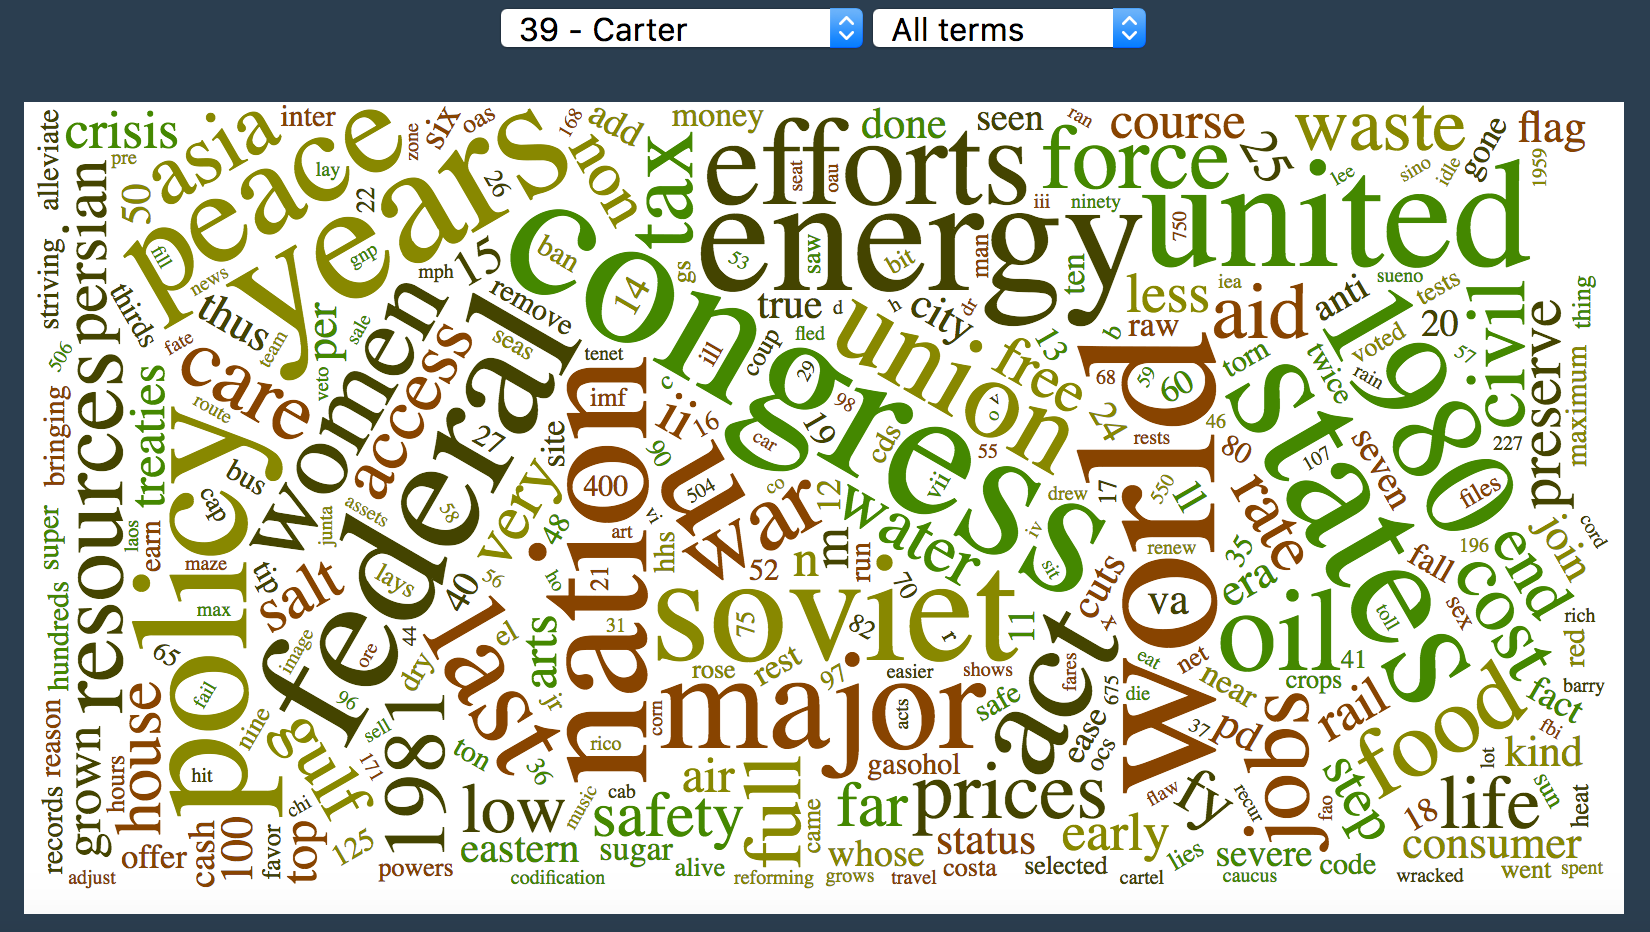
\includegraphics[width=\columnwidth]{images/Wordcloud.png}
  \caption{Example Word Cloud showing all terms for Jimmy Carter}
  \label{fig:wordcloud1}
\end{figure}

\begin{figure}
  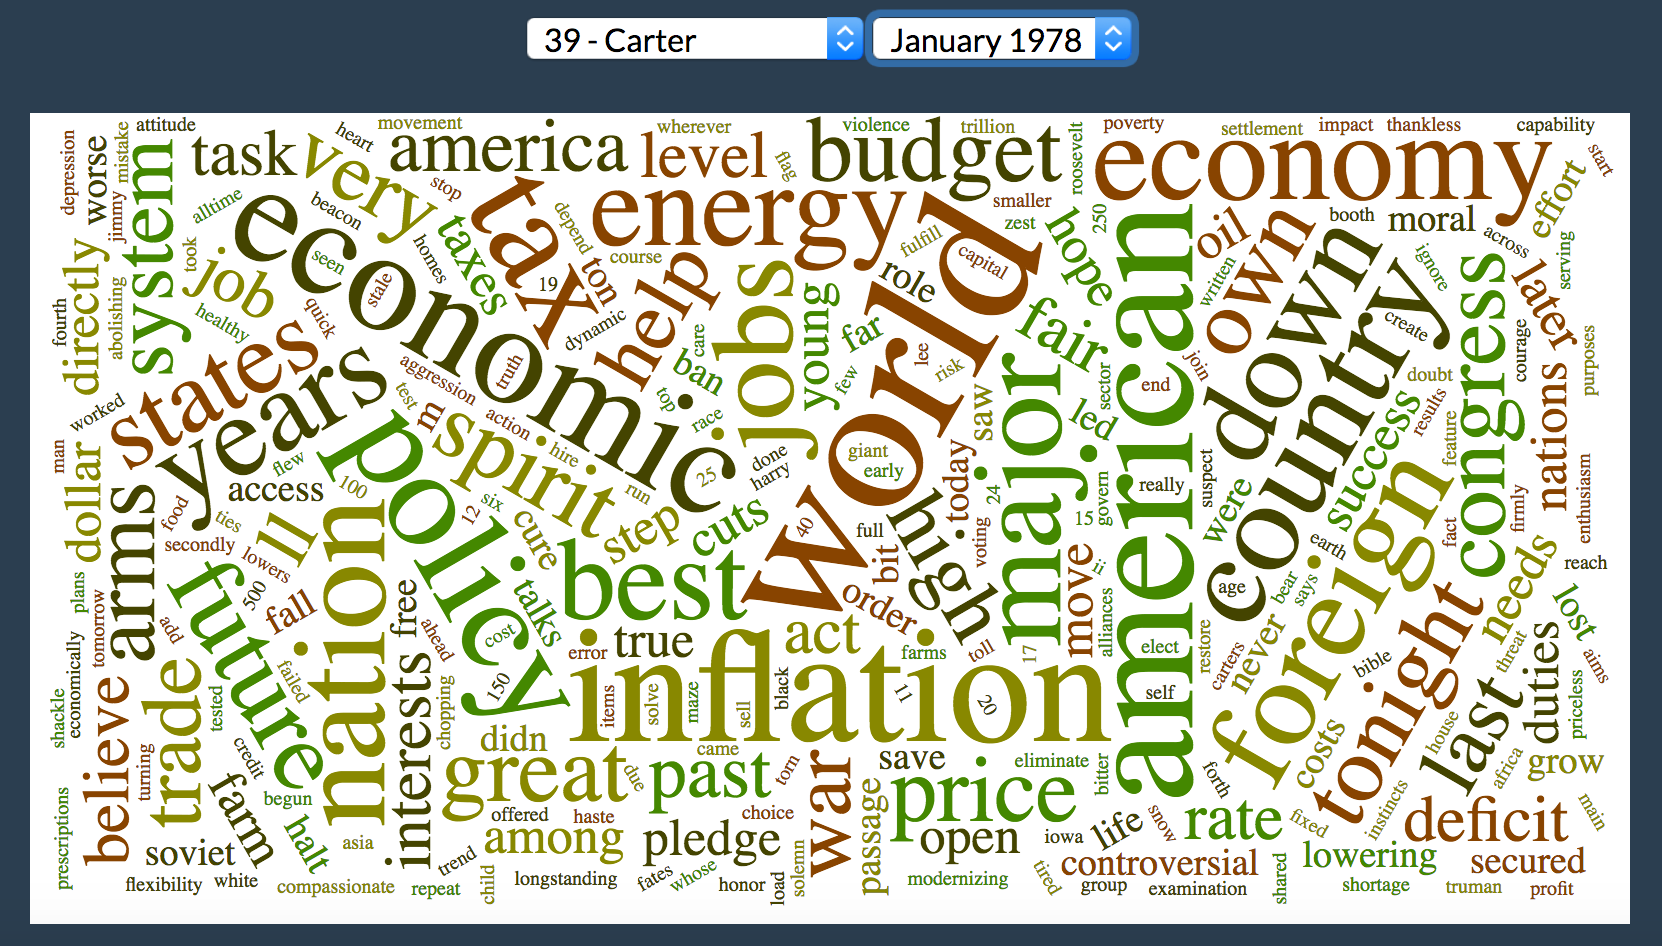
\includegraphics[width=\columnwidth]{images/Wordcloudterm.png}
  \caption{Example Word Cloud showing 1978 term for Jimmy Carter}
  \label{fig:wordcloud2}
\end{figure}

\subsection{D3}
D3.js (D3) is the JavaScript Library used to create the visualization mentioned in the previous section and another mentioned in a future section.
D3 uses pre-built JavaScript functions to select, elements, create SVG elements, style them, or add dynamic effects or tooltips to them [\cite{bostock2011d3}].
D3 also has a handy library that creates word clouds that was used in this research, it takes in an input array in JSON format with the words and their frequencies in decreasing order and draws the words with their relative sizes on the HTML canvas.
There is a bit of a delay on the drawing of the word clouds, since instead of saved images of the word clouds, the program is actually drawing all of them in realtime and just swapping out the JSON data source depending on which President is selected in the dropdown menu at the top of the page.

\section{Results}
The bulk of this information is used later for processing, but it is important to understand the data source as well, before diving in to predictions using it.
The importance and purpose of the State of the Union address is important here since it has a heavy-handed influence on the content and message behind the Presidential Addresses.
It is important to note that the party breakdown, with 26 Republicans and 16 Democrats, makes their percentages 62\% and 38\%, respectively.
These numbers aren't exactly correct, as the lesser-known and ephemeral early parties were placed in to either Democrat or Republican based on their policy positions.
For example, Democratic-Republicans were assigned Republican as that party eventually became the common day Republican party, and the Whig Party was assigned to Republican as well as it was created from former of the Democratic-Republican Party.
This was done in order to maximize the effectiveness of the prediction algorithm that will be discussed later on.
The statistics here are important as they provide more insight into the data being processed and provide a more concise view into what is being handled.
Table \ref{stat:one} has some intriguing patterns and trends to analyze and show.

\subsection{Average Address Length}
The average length of the Presidential Address has changed drastically over time, as its purpose and importance fluctuated.
George Washington, when he gave his first address, didn't think that it would be a reoccurring event, but thought it necessary to inform the citizens of the current state of affairs of the country, and this precedent was followed for much of the early history of the United States [\cite{freeman1948george}].
The relatively short length of the early Presidential Addresses shows this, as it was short and brief.
It was meant to inform the people of what is happening in the country and was used primarily to disperse information to the citizens.
This slowly began to change over the years and the change can be seen in just the average number of words in the addresses.
This change indicates the increasing importance of the State of the Union address as a chance to communicate with the citizens at large and use that attention to push an agenda and connect with the voters.
The State of the Union address became a much larger deal as President's used it to communicate with the entirety of the nation to ensure them of the success of the nation and its status, peaking with Theodore Roosevelt averaging almost 20,000 words per Presidential Address.
Shortly after, however, the length of the addresses had a tremendous drop-off from Taft at 17,000 words to Woodrow Wilson at 4,300 words, which can likely be attributed to the emergence of World War I.
The country was involved in a major war effort and the fanfare and policy pushing of State of the Unions past were cleared out of the way for the focused messages of State of the Union addresses to come.
These were defining times in the world, and with a major conflict to unite all people in the country, the State of the Union addresses became more condensed and focused on the important aspects at hand.
These shorter addresses were used to encourage the country and assure them of the success of the war effort and keep country-wide morale high and trying not to distract them for too long.
From this major change and in to the modern era, the State of the Union address has stabilized around 5,000 to 10,000 words, keeping to an average length and the TV equivalent of roughly an hour to an hour and a half, long enough to keep people's attentions and effectively convey a president's reflections on the past year and goals for the next.

\subsection{Lexical Diversity}
Lexical Diversity, which was introduced previously, is also interesting to note here and it generally follows the same pattern as average length, just in the reverse fashion.
As one would expect, the more words that are spoken, the less overall unique words are going to be spoken.
This is most evident when examining the lexical diversity of George Washington and that of Teddy Roosevelt.
George Washington had notoriously short State of the Union Addresses so his average lexical diversity was 0.3762, whereas Teddy Roosevelt has an average lexical diversity of 0.1732, which makes sense since his average length is almost ten times greater than that of George Washington's.
This provides more important insight in addresses that are similar length to one another and provides a deeper insight into the speech-writing process and how word selection is important when communicating information to large swathes of people and needing to be considerate of their education levels.

\subsection{Grade Level}
Another metric that complements Lexical Diversity that needs to be considered is Grade Level, which was mentioned previously and it is computed using the Flesch Kincaid mentioned above.
The scores seen here may seem rather high but it is understandable given the change in how Americans speak over time.
Speakers in Early America were known to have a rather complicated way of talking and in order to make it to the office of President one had to be sufficiently educated to get elected by the public.
This pattern shows in the high grade level throughout the early and mid history of the United States as most of the early presidents were college-educated, a rarity of the time, and had a more sophisticated vocabulary than the common man.
Also the early speeches were often given in front of Congress and with no means of distributing the speech widely, the intended audience was mainly Congress, so the early Presidents did not really have a need to simplify their language to communicate effectively to the common man as was done by the newspapers that talked about the Address [\cite{ziff1991writing}].
The grade level gradually has decreased over time, which has as much to do with the greater reaches the address has, as it does with the way modern day media collects sound bites of presidential addresses.
In the modern era, when a President gives a speech, only a small amount of the actual speech is rebroadcast when the media is discussing it, so the ``sound bite" phenomenon has arisen in State of the Union addresses, which has had a transitive effect on the Flesch-Kincaid grade level calculation.
The media only takes small snippets of what the President says to convey major policy positions, which has had the effect that most statements are kept short in order to summarize points and clearly convey what positions the President has in as short a form as possible [\cite{paletz1977presidents}].
And since one of the calculations for the grade level calculation is average words per sentence, this brings down the grade level of the speech as the President attempts to become more clear in their purpose and position to effectively convey their thoughts and feelings in a short sound bite that could be taken from their speech.